
\documentclass[journal,onecolumn,11pt]{IEEEtran}

\usepackage{graphicx}
\usepackage{hyperref}
\usepackage{caption}

\ifCLASSINFOpdf

\else

\fi


\usepackage{url}
\usepackage{amsmath}
\usepackage{dirtytalk}
\usepackage{subcaption}

\hyphenation{op-tical net-works semi-conduc-tor}


\begin{document}

\title{Event Prediction using Machine Learning Techniques}

\author{M.Tech~Project~Report\\
        Rohan Sonawane (CS17M066),~\IEEEmembership{M.Tech~Scholar,~IIT Madras.}% <-this % stops a space
\thanks{}% <-this % stops a space
\thanks{}% <-this % stops a space
}

\maketitle

\begin{abstract}
In everyday at each moment various events are happening around us. The events are temporal i.e there is importance to the sequence of the events. The events which happens are related to each other. Events generally follows cause effect relationship. It is very interesting to find the cause of the particular event. In the work presented below our focus is to find the cause of the events i.e relationship among the events. In the following work as a first step towards solution of our problem the machine learning technique Random Forest is used for finding responsible organization for attack. Global Terrorism Database is used which contains more than 150000 records about terrorist attacks. In parallel the knowledge about attacks and terrorist organizations is represented as Ontology. The queries on the ontology can give some meaningful information which will help for better prediction accuracy.
\end{abstract}

% Note that keywords are not normally used for peerreview papers.
\begin{IEEEkeywords}
Random Forest, Ontology, Prediction, Causality pairs
\end{IEEEkeywords}

\IEEEpeerreviewmaketitle



\section{Introduction}
\label{intro}
In our everyday life different occurrences happen around us. Each occurrence has a timestamp and nature. These occurrences are denoted by term "Event". The formal definition of event is occurrence happening at a specific time and place, with or without the participation of human agents . The event may be a part of a chain of occurrences as an effect of a preceding occurrence and as the cause of a succeeding occurrence \cite{def}.
Example : The earthquake of Richter magnitude scale 8 and above has happened at the sea bed. As an effect of the earthquake tsunami hits the sea shore.
In this particular chain of events, the tsunami is the event created by the large magnitude of earthquake.
 The interesting problem to solve here is, given a magnitude of earthquake and the location information, the function will give tsunami alert warning. There is a system where earthquake sensors are deployed all over the place. After sensing the earthquake information, our function will predict whether tsunami will occur or not. The system is useful in areas near coast for tsunami alert. The database used in this task is the information obtained from seismometer and the location information. Another problem of interest is given the tsunami has occurred, find the cause events because of which tsunami has occurred. The task is performed by doing intelligent reasoning on database about events recorded with time-stamp. The example mentioned about is just about one domain. Similar problems problems can be solved which causes social instability like terrorist events. The domain of our interest is events related to military operations. In military locations there are lot of events which has very good correlation with each other. For example : The event \say{Terrorists infiltrated in State} is the cause of the event \say{Firing happens in the state.} There are many events which follows cause-effect relationship. For example : Is the given inflammatory speech by some person is a cause of some terrorist attack or violence?



\begin{figure}[h!]
    \centering    
    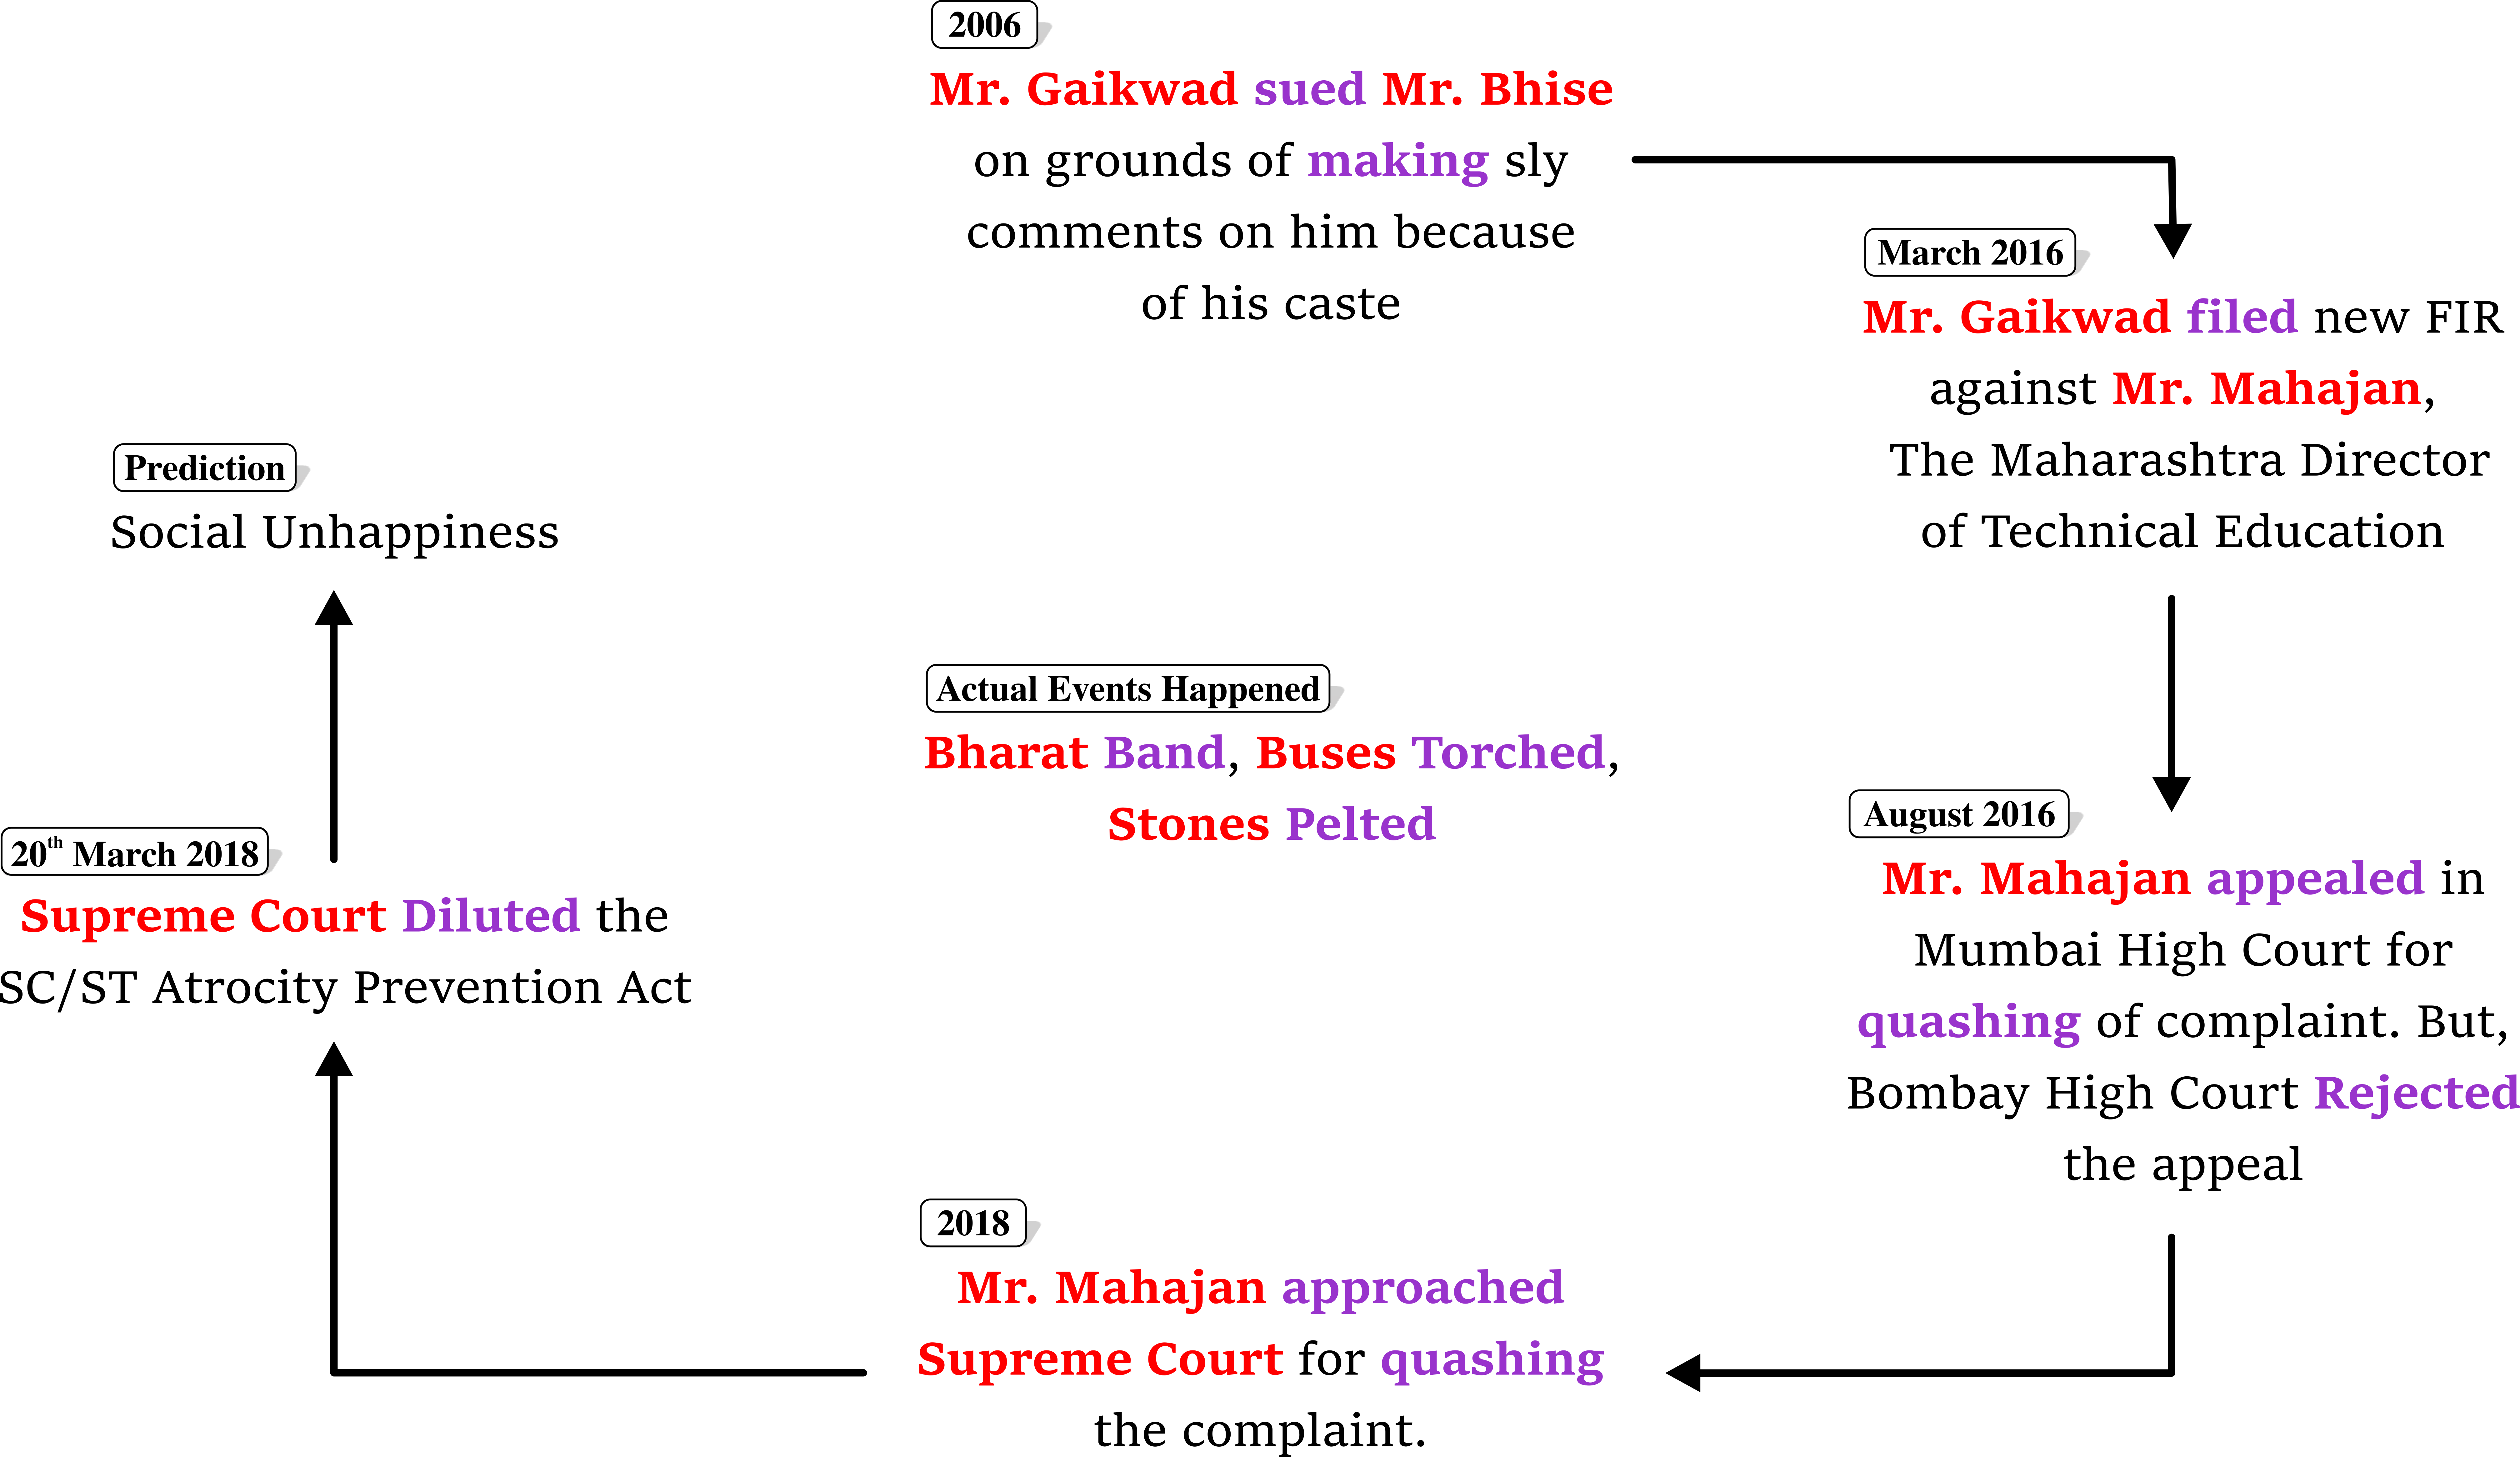
\includegraphics[scale=0.5]{new2_PNG.png}
    \caption{Example of Cause-Effect Relationship of Events}
\end{figure}
\newpage
The given example is latest events chain about Dilution of SC/ST Atrocity Prevention Act \cite{news}. It started in 2006, when Mr. Gaikwad filed a case against his supervisor for complaining about his performance because of his caste not because of performance. After 10 years, Mr. Gaikwad again filed an FIR against Mr. Mahajan because he did not take action on his first complaint.  Mr. Mahajan in August 2016 went to High Court for quashing the complaint. But High Court dismissed his appeal as effect he went to Supreme Court. Supreme Court on hearing of his case diluted the SC/ST act on March 20, 2018. So as people are very sensitive about this issue, our system should predict that \say{There will be social unhappiness in the society}. \\
\indent In this example there is a condition of social unrest. Here the event prediction system is useful to avoid loss of property and life. The data sources from which information is extracted are the print-media, Online news portals. This example is different from the tsunami prediction example, because in this example the data from which events are extracted is unstructured data. IT is difficult to extract the events because there are large number of data sources from which information can be extracted. Another difference is in the tsunami prediction example we can easily predict the event that the tsunami will occur. But in the second example it is very difficult to predict the what exactly can happen. Social unhappiness can mean different things like riots can happen or protest can happen. The problem of interest is the system should perform forward prediction as well as backward prediction. In the second example if the event given is \say{Social unrest in society.} the system should be able to find the causes of this event.\\
\indent In the literature, research has been done about modeling the event in structured format and predict the cause-effect relationship among events. They extracted news headlines from newspapers and structured the event in the format given below. The details about their work is mentioned in the literature survey \autoref{lit}.
In the following diagram the formalization of event is shown and the strength of the caused events is predicted by algorithm using the data.

\begin{figure}[h!]
    \centering
    \def\svgwidth{0.8\columnwidth}
    
    \input{cause_effect_new.pdf_tex}
    \caption{Pair of Events having Cause-Effect Relationship}
\end{figure}
\newpage
First event from natural language is converted to structured format i.e Action, Actor, Location, Instrument and the object on which action is performed is extracted. The next step is to find relationship between object of one event to object of another event. For this task linked open data can be used. Examples of linked open data are DBpedia, WordNet, Yogo, Freebase etc. By building abstraction tree where nodes represents events prediction is preformed. The important challenge in this task is to extract the events. There is huge information about events presents in various forms like newspapers, news channels, blogs, videos of speeches etc. The information available is highly unstructured.\\
\indent The motivation behind building this prediction system is to learn from scratch how to build an event prediction system. In discussion with people who are in this field, such softwares are charged very heavy amount of money by multinational companies causing the loss to company. The system will help our country to reduce the risk of terrorist attack significantly.

The domain under study is terrorist events prediction. The database used for this task is Global Terrorism Database (GTD). Global terrorism database is available which contains more than 150000 terrorist events recorded with details. Our idea is to build a forward as well as  backward prediction. Backward prediction includes, given an event find the cause events for the event. In addition to building predictor, we have build an ontology related to terrorism events. The ontology contains detailed classification about terrorism domain. The purpose of building ontology is to extract the relationships between objects in the events. By using ontology we can able to query some intelligent questions about terrorist attacaks. In the literature people have classified the database and build the model to predict the weapontype, attacktype, targettype of terrorist attacks. The detailed information is given in the literature survey. The detail similar work performed in this domain is mentioned in Literature Survey \autoref{lit}. In the third chapter, our solution is proposed \autoref{solution}. In fourth chapter Experimentation and Results \autoref{experiment}are mentioned. In the fifth chapter Future Scope \autoref{future}of the project is mentioned.
% \subsection{How can we get the events?}
% The important task is to find the events from the stream of various data sources. This task is difficult because the information is unstructured data. The data sources can be national and local news articles, heated speeches information, blogs about terrorism events, Portals on Internet which gives information about terrorist attacks, Terrorist Organizations etc. But it is not easy to extract the events from natural language description. For this task we need to use NLP techniques to convert the news in the format of event we have defined. The tasks involved in this step are crawling the web for getting news and using NLP parsers to find the nouns, verbs, adjectives and map them to appropriate object in tuple of event.


\section{Literature Survey}
\label{lit}
Similar work in this field is done. Some of them is mentioned below:
\subsection{Learning to Predict from Textual Data}
The forward prediction of events is done by students at Israel Institute of Technology using causality pairs\cite{paper1}. Causality pair is the pair which contains cause effect and corresponding effect event. The focus of the research is on the extracting the causality and predicting the event based on it. The basic idea is to crawl the headline of the news article and find the cause and effect pairs from each headline. Then we find the events which are causes of other 
events. They have found very elegant way to represent the evevnt in structured format which is defiend below: \\ $E = < P, O_1, O_2, O_3, O_4,t >$
\begin{itemize}
    \item P is a temporal action or state that the events objects exhibit.
    \item $O_1$ is the actor that performed the action.
    \item $O_2$ is the object on which the action was performed.
    \item 	$O_3$ is the instrument with which the action was performed.
    \item $O_4$ is the location of the event.
    \item 	t is a time-stamp.
\end{itemize}



The algorithm works in a way that given event in natural language, it will produce the events it can cause (textual causality patterns). The result is a graph with node represents facts. Here child will be the effect of the parent node.  The learning algorithm uses large ontologies to generalize the events and predict the causality of unseen events. The algorithm uses the concept of generalized path which finds the relationship between the objects and store it.
When new object in cause event comes using the rule it will find the effect object.

\begin{figure}[h!]
    \centering
    \def\svgwidth{\columnwidth}
    
    \input{new1.pdf_tex}
    \caption{Event Predictor based on Causality Pair Extraction}
  
\end{figure}

The data used is from past 150 years. To extract training examples textual causality patterns are used.\\
Example : The pairs are of the form $(Y, X)$ if \say{$X$ because $Y$} or $(Y, X)$ \say{$X$ causes $Y$}.
Some real world examples are:
If the given event is \say{Magnitude 6.5 rocks the Solomon Islands} then the prediction is \say{A tsunami warning will be issued for the Pacific Ocean.}It has inferred from the following pair in the event database:\\
$<$7.6 Earthquake strikes island near India, Tsunami warning issued for Indian Ocean$>$\\
The algorithm works in following way:
\begin{enumerate}
    \item First we extract the causality pairs from the data-sources. Here data-source used is news from NewYork Times Newspaper.
    \item Then we generalize using world ontology and produce abstraction tree. Here generalization means if in the news if \say{Japan} is mentioned the system should understand that it is a name of the country.
    \item All the similar events are clustered and represented as one node in abstraction tree. For each node prediction rule is generated from the examples in the node.
    \item When new event comes, it gets match to the node in the abstraction tree and the stored rule is applied to find the effect event.
\end{enumerate}

Now lets understand what is the representation of event.
The event is represented by three methods:
\begin{enumerate}

\item Event at sentence level. Event similarity is calculated using bag of word model. The number of similar words in sentence describes the similarity of two events.
\item Second approach is semantic, In the second approach the words in the sentence are transformed to noun-phrase.
\item Third approach is semantic, This approach maps  each element in event to a semantic concept.\\
For example :  "The US Army Destroyed the warehouse in Iraq with explosives". The date of the event is October 2004. 
It is modelled as  Destroy(Action), US Army(Actor), warehouse(Object), explosives(Instrument), Location(Iraq), October 2004(Time).
\end{enumerate}
In this algorithm for representation of events third approach is used. After representing the events the main challenge is to generalize the objects and actions in the events which will get used in prediction. Generalization means if there are two training examples $<$earthquake in Turkey, Destruction$>$ and $<$Earthquake in Australia, Destruction$>$ When new event comes $<$earthquake in Japan$>$,
from Turkey and Australia algorithm should understand that Japan is also a country. So prediction should be "Destruction". 

To generalize objects Linked Open Data is used where the nodes are objects in the universe for example nouns and the edges are relations or verbs. Two objects are said to be similar if they relate third object in the same way.
For example : Delhi and Beijing are similar objects because they are related to the Asia in the same way  $capitalOf \xrightarrow{} InContinentOf$  
The sequence of relations is called the \textit{generalization path}.
We have to consider shortest generalization path which is called \textit{minimal generalization path}.

For all pairs (a, b) in the dataset, algorithm finds node \say{c} such that \say{a} to \say{c} and \say{b} to \say{c} are connected with the same relation set say $(l_1, l_2, \dots, l_k)$. Now by the approach of dynamic programming we consider node \say{x} connecting to \say{a} and node \say{y} connecting to \say{b} with the same label $l$, then the minimal generalization path for \say{x} and \say{y} will be same as minimal path between a and b with the addition of edge $l$.
To describe the relation between verbs the same process is performed except the semantic network used is VerbNet.
dist(a, b) denotes the length of the MGenPath.


\begin{figure}[h!]
    \centering
    \def\svgwidth{0.35\columnwidth}
    
    \input{fig3.pdf_tex}
    \caption{Generalization path}
\end{figure}
The important task is to generalize the event, To provide more generalization we need to find the events which can be represented as the single abstract event. We have to cluster the events so that the events which have same cause and effect comes under same cluster or node. Similarity between two events is given by :\\
$SIM(e_i, e_j) = f(dist^{G_p}_{Gen}(P^i, P^j), dist^{G_o}_{Gen}(O^i_1, O^j_1), ..., dist^{G_o}_{Gen}(O^i_4, O^j_4)) $\\
Here $f$ is the aggregation function which is chosen as average.
Similarity between pairs of cause and effect will be given by:\\
$SIM(<c_i, e_i>,<c_j , e_j>) = f(SIM(c_i,c_j ), SIM(e_i, e_j))$\\
In abstraction tree all the events which are similar are represented by one node. For each node  among all the events there is a one event which is representative event of the node.

Next step is to create the prediction rule. We need to abstract the relationship between the cause and effect and create a prediction rule. For example \say{Earthquake hits turkey} is the cause effect and \say{Red cross help sent to Ankara} should be abstracted as \say{Earthquake hits [Country Name]} and effect will be \say{Help sent to [Capital of Country]}. Now it is important to understand how to learn these clauses automatically. It is divided in two steps:
\begin{enumerate}
\item Find the path from objects of cause effect to object from effect event of length at most k. here k is the parameter.
\item Construct the clause using labels of the 
path as predicates.
\end{enumerate}

We find path from the object of cause event to any other object of the effect event. 
After finding the path we store the path. When new event comes, we apply the projection of path to get effect object. k is hyper-parameter. To find k, for each training example in node we find all paths with increasing values of k. Then the path which is mostly seen is considered as the final path and value of k corresponding to path is considered as optimal value of k.

At the time of actual prediction we have a cause event. The algorithm starts from the root of the tree and and find the similarity between representative cause event of node and the given event and expand the search if  children of the node has better similarity.
After retrieving the node we apply the projection rules of predicates and find the possible effect events. We may get more possible effect events because of different predicates.
So after generating each effect event we find its similarity with effect event of the node and sort the events and pick the one who is most similar to the effect event of node. This algorithm predicts the events with the accuracy 63\%.
Following are the results of the algorithm and comparison with human prediction.
\begin{table}[h!]
\centering
\fontsize{11}{9}\selectfont
\bgroup
\def\arraystretch{1.5}
\begin{tabular}{|l|l|l|}
\hline
\textbf{Event} & \textbf{Human-predicted event} & \textbf{Pundit-predicted event} \\ \hline
Al-Qaida demands hostage exchange & Al-Qaida exchanges hostage & A country will refuse the demand \\ \hline
\begin{tabular}[c]{@{}l@{}}Volcano erupts in Democratic Republic\\ of Congo\end{tabular} & \begin{tabular}[c]{@{}l@{}}Scientists in Republic of Congo \\investigate lava beds\end{tabular} & \begin{tabular}[c]{@{}l@{}}Thousands of people flee from\\ Congo\end{tabular} \\ \hline
\begin{tabular}[c]{@{}l@{}}7.0 magnitude earthquake strikes\\ Haitian coast\end{tabular} & Tsunami in Haiti affects coast & Tsunami-warning is issued \\ \hline
\begin{tabular}[c]{@{}l@{}}2 Palestinians reportedly shot dead\\ by Israeli troops\end{tabular} & \begin{tabular}[c]{@{}l@{}}Israeli citizens protest against\\ Palestinian leaders\end{tabular} & War will be waged \\ \hline
\begin{tabular}[c]{@{}l@{}}Professor of Tehran University\\ killed in bombing\end{tabular} & \begin{tabular}[c]{@{}l@{}}Tehran students remember slain \\professor in memorial service\end{tabular} & Professor funeral will be held \\ \hline
\end{tabular}
\egroup
\caption{Results of Pundit Algorithm}
\end{table}
\subsection{ Future Terrorist Attack Prediction using Machine Learning}
In this work the terrorist attacks are predicted from the past data about terrorist attacks all around the world \cite{paper2}. The machine learning technique used here is called random forest. Random forest is an algorithm where the entire data is split into subsets of data. The classifier is a decision treee which takes input and provides the class label as output. Instead of having one strong tree, the technique uses many weak trees as a base classifier. All the decision trees are trained using the subsets of data provided to them. After training, at the time of testing, sample data point feeds to all the trees and voting technique is applied to find the final class.

Following are some advantages of random forest:
\begin{enumerate}
\item Used both for classification and regression
\item Handle missing values and maintain accuracy for missing data.
\item Won't overfit the model.
\item Higher large dataset with higher dimensionality.
\end{enumerate}
The disadvantage of Random Forest is that it is good for classification, but not as good for regression.\\
All sample examples are classified into two sets 70\% training set and 30\%testing set. Based on the number of examples the number of decision trees in the forest are decided. Random samples from training set are used as input for each tree. Here we need to make sure that the set of examples selected for each forest should be different from each other. Otherwise each decision tree will learn the same pattern and we will not get accurate results.  The errors in the learning process are mainly Variance, Bias and Noise. But Bagging minimizes all the errors. The variance in of data is reduced by Ensemble technique.

Whether to use regression or classification depends on the nature of the data. If we have discrete data in classes we can use classification . But if the data is continuous we use regression. In this case classification gives better results than regression as the data is discrete.

The data selected for this task is Global Terrorism Database(GTD). After performing dimensionality reduction the features selected are Location, AttackType, WeaponType, TargetType. In the ensemble learning phase it should take two parameters: \say{the number of attributes trees should consider} and \say{number of trees}. After training Accuracy, Sensitivity and Specificity is calculated using test data.
The learning algorithm used is both random forest classification and random forest regression but random forest classification gives better result than random Forest Regression. 
When attackType is the field to predict, other fields like location, weaponType, targetType are considered as features or input sample data.  The accuracy obtained is 76\% - 79\% for attackType. Similarly if weaponType is considered for prediction  the accuracy obtained is 84\% - 86\% and for targetType 33\% - 36\% accuracy is obtained.

\section{Our Solution}
In the proposed solution for each event, we are interested in the weight of the cause events. The following diagram explains details about it.


\label{solution}
\begin{figure}[h!]
    \centering
    \def\svgwidth{0.35 \columnwidth}
    
    \input{fig1.pdf_tex}
    \caption{Event Chain}
\end{figure}

The diagram above shows how events are related to each other. Here $E1, E2, E3, E4, E5$ are some events which are correlated to each other i.e there is cause effect relationship among them. This is the expected model which will tell the cause of event with the weight which shows importance of cause. Here Event E4 is caused by two events E1 and E2 in which E2 is more responsible for E4 to happen. So in future when if one of the event happens by analyzing the probabilities associated with the effect events we can tell the possible future event.

The proposed system architecture is given below:


\begin{figure}[h!]
    \centering    
    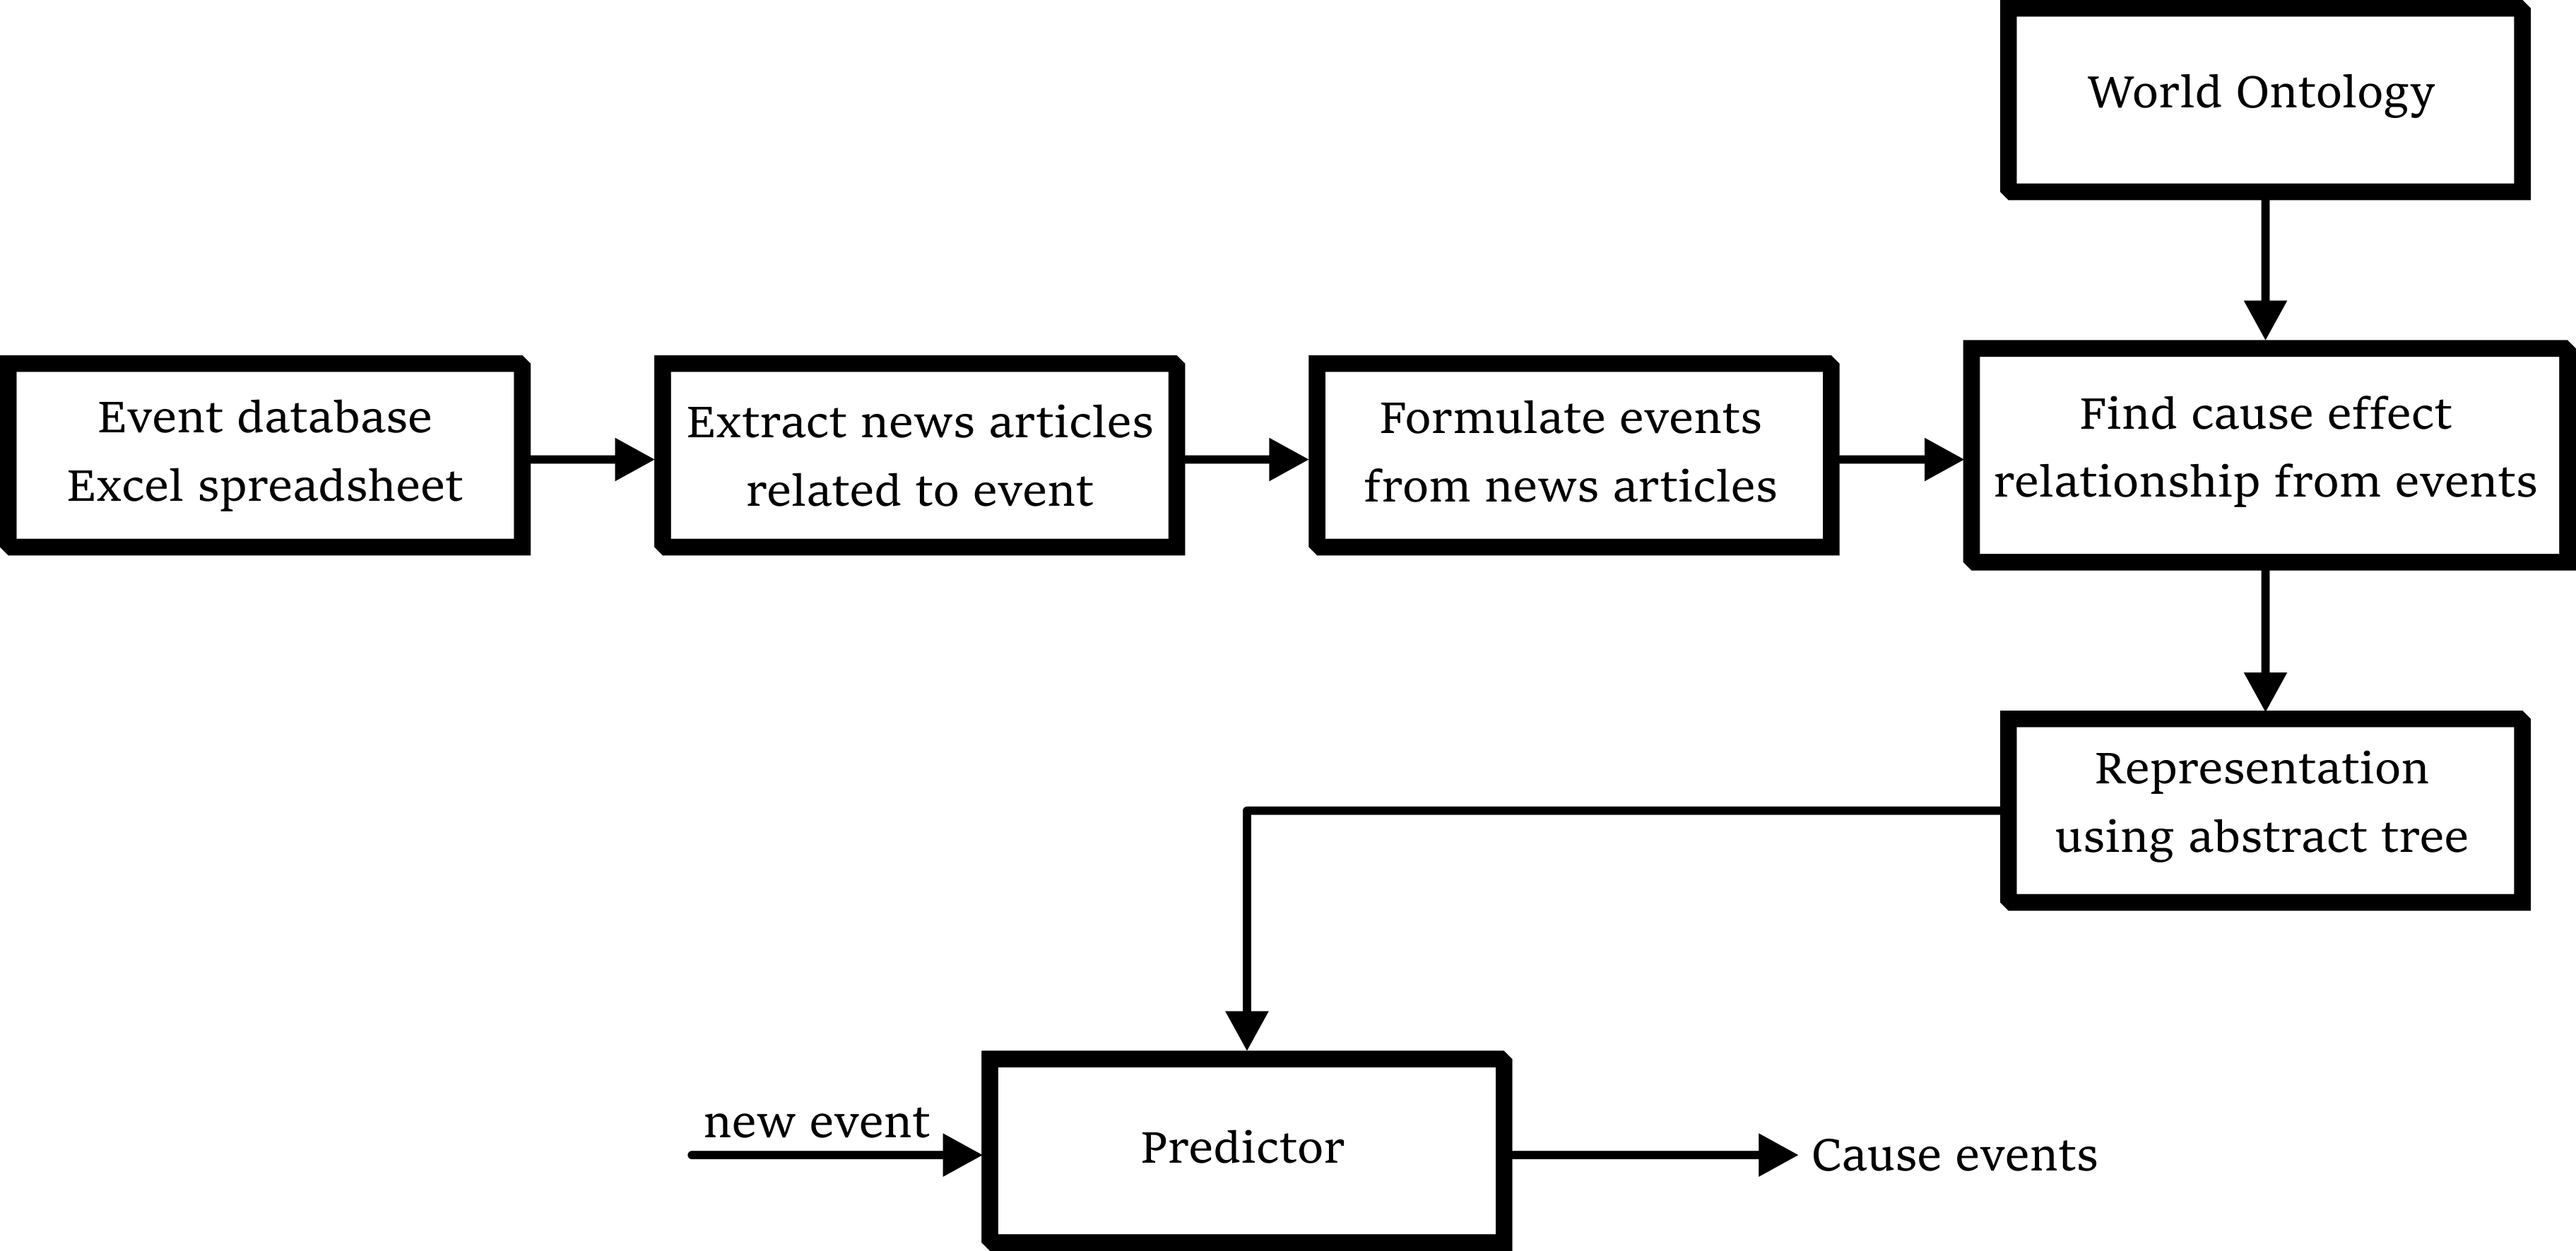
\includegraphics[scale=0.8]{architec.png}
    \caption{Example of Cause-Effect Relationship of Events}
\end{figure}

Input data is a spreadsheet of events from Global Terrorism Database. For each event we will extract the news articles in the date range of given event (articles before and after 15 days of event date). From news articles extract the events and formulate them as tuple mentioned in the literature survey. After extraction events, we will find cause-effect relationship among events using ontology. After finding cause effect relationship between events, we will represent in the form of tree. where parent is cause event and child is effect event.     

The datasets which are identified are:
\begin{itemize}
\item Global Terrorism Database
\item Big Allied and Dangerous Database (Contains information about all terrorist organizations)
\item South Asia Terrorism Portal
\item Local Newspapers in Kashmir eg. Rising Kashmir, Greater Kashmir etc.
\item News sources of neighboring countries
\end{itemize}

To initialize the Global Terrorism Database is used because it is structured dataset. The problem that is going to be address is finding the cause-effect relationship among the events. To find the relationship among events the knowledge should be represented in the form of machine interpretable format. This is the motivation for developing the ontology for the terrorist attack events. Following is the information about some datasets :\\ \\
\textit{Global Terrorism Database} : It is an open source database which includes detailed information about terrorist attacks from all over the world from the 1970 to 2017. It is collected and maintained by University of Maryland. In contains around 1,80,000 terrorist attacks. To obtain this data 40,00,000 news articles and 25,000 news sources are utilized. Some of the important fields are given below: \cite{gtd} \cite{gtd codebook}\\

\begin{table}[h]
\fontsize{11}{9}\selectfont
\bgroup
\def\arraystretch{1.5}
\begin{tabular}{|l|l|l|}
\hline
\multicolumn{1}{|c|}{\textbf{Property}} & \multicolumn{1}{c|}{\textbf{Column Name}}                              & \multicolumn{1}{c|}{\textbf{Description}}                                                                                                                                                                                                                                                                                                                                                                                    \\ \hline
GTD ID                                  & eventid                                                        & \begin{tabular}[c]{@{}l@{}}12 digit event id {[}first 8 digits represent date “yyyymmdd”  format and next \\four digits are for sequence in a day{]}\end{tabular}                                                                                                                                                                                                                                                           \\ \hline
Year                                    & iyear                                                                  & Year in which incident occurred.                                                                                                                                                                                                                                                                                                                                                                                             \\ \hline
Month                                   & imonth                                                                 & Month in which incident occurred.                                                                                                                                                                                                                                                                                                                                                                                            \\ \hline
Day                                     & iday                                                                   & Day in which incident occurred.                                                                                                                                                                                                                                                                                                                                                                                              \\ \hline
Incident Summary                        & summary                                                                & Summary of the incident.                                                                                                                                                                                                                                                                                                                                                                                                     \\ \hline
Country                                 & \begin{tabular}[c]{@{}l@{}}country\\ country\_txt\end{tabular}         & \begin{tabular}[c]{@{}l@{}}ID of the country code\\ Country where incident has happened\end{tabular}                                                                                                                                                                                                                                                                                                                         \\ \hline
City                                    & city                                                                   & Name of the city where incident has happened.                                                                                                                                                                                                                                                                                                                                                                                \\ \hline
Latitude                                & latitude                                                               & Latitude of the location where incident has happened.                                                                                                                                                                                                                                                                                                                                                                        \\ \hline
Longitude                               & longitude                                                              & Longitude of the location where attack has happened.                                                                                                                                                                                                                                                                                                                                                                         \\ \hline
Attack Type                             & \begin{tabular}[c]{@{}l@{}}attacktype1\\ attacktype1\_txt\end{tabular} & \begin{tabular}[c]{@{}l@{}}One among the following values {[}Assassination, Hijacking, Kidnapping, \\ Barricade Incident, Bombing/Explosion, Armed Assault, Unarmed Assault, \\ Facility/Infrastructure Attack, Unknown{]}\end{tabular}                                                                                                                                                                                      \\ \hline
Weapon Type                             & \begin{tabular}[c]{@{}l@{}}weapontype1\\ weapontype\_txt\end{tabular}  & \begin{tabular}[c]{@{}l@{}}One among the following values {[}Biological, Chemical, Radiological, Nuclear, \\ Firearms, Explosives, Fake weapons,  Incendiary, melee, Vehicle, Sabotage \\ Equipment, Other, Unknown{]}\end{tabular}                                                                                                                                                                                          \\ \hline
Victim Type                             & \begin{tabular}[c]{@{}l@{}}victimtype1\\ victimtype1\_txt\end{tabular} & \begin{tabular}[c]{@{}l@{}}One among the following values {[}Business, Government, Police, Military,\\ Abortion Related, Airports and Aircrafts,  Educational Institutes, Food and \\Water Supply, Journalists and Media, Maritime, NGO, Other, Private Citizen \\and Property, Religious Figures, Telecommunication, Terrorists, Tourists, \\Transportation, Unknown, Utilities, Violent Political Parties{]}\end{tabular} \\ \hline
Perpetrator Group                       & gname                                                                  & Name of the group who has performed the attack                                                                                                                                                                                                                                                                                                                                                                               \\ \hline
\end{tabular}
\caption{Global Terrorism Database}
\egroup
\end{table}
\newpage
\textit{Big Allied and Dangerous (BAAD)} :  It is the database which includes detailed information about the terrorism organizations from 1998 to 2005. It is also maintained by University of Maryland. The important fields related to this database are as follows: \cite{baad}
\begin{table}[h]
\centering
\fontsize{11}{9}\selectfont
\bgroup
\def\arraystretch{1.5}
\begin{tabular}{|l|l|l|}
\hline
\multicolumn{1}{|c|}{\textbf{Property}} & \multicolumn{1}{c|}{\textbf{Column Name}} & \multicolumn{1}{c|}{\textbf{Description}}               \\ \hline
Group Name                              & group                                     & Name of the terrorist Organization                      \\ \hline
Country                                 & country                                   & Origin country                                          \\ \hline
Number of Allies                        & no of allies                              & Number of organizations which supports the organization \\ \hline
Number of rivals                        & no of rivals                              & The rivals of the particular organization               \\ \hline
Age                                     & age                                       & Age of the organization                                 \\ \hline
Number of fatalities                    & no of fatalities                          & Number of kills they have till date                     \\ \hline
\end{tabular}
\caption{Big Allied and Dangerous (BAAD) database}
\egroup
\end{table}

\section{Experimentation \& Results}
\label{experiment}
The work for this semester is divided in two parts:
\begin{enumerate}
\item Prediction from structured data using machine learning technique Random Forest Classification. In this task the correlation among the features is measured.
\item Representation of knowledge in the form of Ontology.
\end{enumerate}
\subsection{Prediction using machine learning technique}

\begin{figure}[h!]
    \centering
    \def\svgwidth{0.4\columnwidth}
    
    \input{fig4.pdf_tex}
    \caption{Random Forest Classifier}
\end{figure}
\begin{itemize}
\item \textit{Data Selection} : The dataselected here is Global Terrorism Database. The fields of the database are mentioned in the table above.
\item \textit{Feature Extraction} : The real time data is always incomplete or has some noisy data. So for the purpose of our task four features are considered Location of the attack, Weapon Type, Attack Type, Target Type.
\item \textit{Pre-processing} : To perform any machine learning prediction algorithm numeric values are very useful and important. So in preprocessing the data about Attack Type, Weapon Type, Location, Target Type, Perpetrator (Attacking organization) is enumerated (stored as a dictionary).
\item \textit{Ensemble Learning} : Ensemble learning use multiple learning algorithms for prediction to obtain better results than any algorithm alone. Here different trees are build using different subsets of data and majority voting technique is used to get the prediction.
\item \textit{Prediction} : The entire data is divided into 70 \% training data and 30 \% test data. The model is trained using the 70 \% of the data and the correctness and accuracy of the model is tested on remaining 30 \% of the data.\\
The highest accuracy obtained is 79.49\% on train data and 43.84\% on test data. Following are the plots about Change in Training and Testing(Validation) Error) with value of k.
%===========================================================

\item \textit{Results}\\
Features selected as an input to algorithm must have less correlation. Following is the correlation between the selected features from the Global Terrorism Database.



\begin{table}[h!]
\begin{tabular}{|l|l|l|l|l|l|}

\hline
 & \textbf{Location} & \textbf{AttackType} & \textbf{Perpetrator} & \textbf{TargetTpe} & \textbf{WeaponType} \\ \hline
\textbf{Location} & 1.000000 & 0.052832 & 0.272303 & 0.030255 & -0.022715 \\ \hline
\textbf{AttackType} & 0.052832 & 1.000000 & 0.008908 & 0.003336 & 0.024838 \\ \hline
\textbf{Perpetrator} & 0.272303 & 0.008908 & 1.000000 & 0.079512 & 0.042912 \\ \hline
\textbf{TargetType} & 0.030255 & 0.003336 & 0.079512 & 1.000000 & 0.604990 \\ \hline
\textbf{WeaponType} & -0.022715 & 0.024838 & 0.042912 & 0.604990 & 1.000000 \\ \hline
\end{tabular}
\centering
\caption{Correlation among features}
\label{my-label}
\end{table}


\begin{figure}[h!]
    \centering
    \def\svgwidth{0.5\columnwidth}
    
    \input{plot.pdf_tex}
    \caption{Correlation among features}
\end{figure}

% \textbf{Input(Features)}                            & \textbf{Output (label)} & \multicolumn{2}{l|}{\textbf{Accuracy}}         \\ \hline
%                                                     &                         & \textbf{Training Data} & \textbf{Testing Data} \\ \hline
% Location, AttackType, WeaponType, TargetType        & Perpetrator Name        &                        &                       \\ \hline
% Location, AttackType, WeaponType, Perpetrator Name  & TargetType              &                        &                       \\ \hline
% Location, AttackType,  TargetType, Perpetrator Name & WeaponType              &                        &                       \\ \hline
% Location, WeaponType, TargetType, Perpetrator Name  & AttackType              &                        &                       \\ \hline
% \end{tabular}
% \end{table}
\end{itemize}

In the first experiment, WeaponType is predicted given the other features Location, Perpetrator Name, AttackType, TargetType. To measure the performance of the model we have evaluated on various performance metric:\newline
\begin{enumerate}
\item Accuracy : It is the ratio of correctly classified examples to the total number of examples.
\item Precision : $\frac{TP}{TP + FN}$
\item Sensitivity : $\frac{TP}{TP +FN}$
\item F1-score : $\frac{2 * (Precision * Sensitivity)} {Precision + Sensitivity}$

\end{enumerate}
\begin{table}[h!]
\centering
\begin{tabular}{|l|l|l|l|l|l|l|l|l|l|l|l|}
\hline
\textbf{Class} & 0 & 1 & 4 & 5 & 6 & 7 & 8 & 9 & 10 & 11 & 12 \\ \hline
\textbf{Precision} & 0 & 0.35 & 0.73 & 0.97 & 0 & 0 & 0.28 & 0 & 0.15 & 0 & 0.8 \\ \hline
\textbf{Sensitivity} & 0 & 0.24 & 0.86 & 0.93 & 0 & 0.66 & 0.14 & 0 & 0.18 & 0 & 0.66 \\ \hline
\textbf{F1-Score} & 0 & 0.28 & 0.79 & 0.95 & 0 & 0.68 & 0.19 & 0 & 0.16 & 0 & 0.72 \\ \hline
\end{tabular}
\caption{Performance measure metric}
\end{table}

\begin{figure}[!htb]\centering
\begin{minipage}{0.4\textwidth}
\centering
\def\svgwidth{\columnwidth}
\input{train.pdf_tex}
\caption{Training Loss Vs Value of k}
\end{minipage}
\begin {minipage}{0.4\textwidth}
\centering
\def\svgwidth{\columnwidth}
\input{test.pdf_tex}
\caption{Validation Loss Vs Value of k}
\end{minipage}
\end{figure}


\newpage
\subsection{Knowledge Representation}
To find the relationship between different objects there is a need of ontological classification of the knowledge of terrorist attacks and information about terrorist organizations. The created ontology will be able to answer the intelligent queries. Following are some examples of queries we can answer:
\begin{enumerate}
\item Which countries have friendly relation with given country?
\item Terrorist attacks where there is no loss of life
\item Terrorist attacks which are executed by organizations whose origin 
\item Population of targeted areas
\item Number of attacks by organizations
\end{enumerate}
For this task the factbook ontology created by CIA \cite{factbook} is extended. The datasource used is mentioned above which is Golbal Terrorism Database (GTD) and Big Allied and Dangerous (BAAD). To extract these events of terrorist attacks, scripts are written in java language. Modifications are performed on the top of existing code from github \cite{github} hich has done the work of extracting terrorist events. The major challenge in the program is that the layout of web has changed. So every minor change is performed to crawl the data. 
The present ontological classification is able to answer only few of the queries. The structure of ontology is given below
\subsubsection{Concepts}
In addition to the concepts in factbook ontology some concepts are added. 
\begin{table}[h!]
\centering
\fontsize{11}{9}\selectfont
\bgroup
\def\arraystretch{1.5}

\begin{tabular}{|l|}
\hline
\textbf{Concept Name} \\ \hline
Attack \\ \hline
AttackType \\ \hline
Country \\ \hline
Perpetrator \\ \hline
VictimType \\ \hline
\end{tabular}
\caption{Concepts in Ontology}
\egroup
\end{table}

\subsubsection{Properties}
\begin{itemize}
\item Object Properties - Two individuals are related to each other using Object Properties. Following are some object properties.
\begin{table}[h!]
\centering
\fontsize{11}{9}\selectfont
\bgroup
\def\arraystretch{1.5}

\begin{tabular}{|l|l|l|l|}
\hline
\textbf{Property Name} & \textbf{Domain} & \textbf{Range} & \textbf{Inverse Relation} \\ \hline
belongTo & Perpetrator & Country & hasPerpetrator \\ \hline
border & Country & Country &  \\ \hline
executedBy & Attack & Perpetrator & executes \\ \hline
hasVictim & Attack & VictimType & isVictimOf \\ \hline
occured & Attack & Country & sufferedFrom \\ \hline
ofType & Attack & AttackType & hasAttack \\ \hline
\end{tabular}
\caption{Object Properties in Ontology}
\egroup
\end{table}
\item Data Properties - Data Properties relate individuals  to literal data (example : strings, numbers, date-types etc.)
\end{itemize}
\newpage
\section{Future Work}
I will implement the proposed system. Expansion of Ontology to include information about countries and their details.
\label{future}
\section{Acknowledgement}
I would like to thank Prof. Narayanaswamy N S to help me and provide me valuable guidance.



% Can use something like this to put references on a page
% by themselves when using endfloat and the captionsoff option.
\ifCLASSOPTIONcaptionsoff
  \newpage
\fi



\begin{thebibliography}{1}

\bibitem{paper1}
Kira Radinsky \& Sagie Davidovich \& Shaul Markovitch, \emph{\say{Learning to Predict from Textual Data}}, Journal of Artificial Intelligence Research 45 (2012) 641-684.

\bibitem{paper2}
Snehanshu Saha \& Abu Kurian \& Aparna Basu , \emph{\say{Future Terrorist Attack Prediction using Machine Learning Techniques}}, https://www.researchgate.net/publication/317032840.

\bibitem{gtd codebook}
Codebook of GTD
\bibitem{gtd}
https://www.start.umd.edu/gtd/
\bibitem{baad}
https://www.start.umd.edu/baad/database
\bibitem{news}
https://www.indiatoday.in/india/story/sc-st-act-from-dilution-to-restoration-in-5-months-1303463-2018-08-02
\bibitem{random forest}
https://medium.com/machine-learning-101/chapter-5-random-forest-classifier-56dc7425c3e1
\bibitem{}
http://dataaspirant.com/2017/06/26/random-forest-classifier-python-scikit-learn/
\bibitem{github}
https://github.com/Dommicentl/FactbookParser
\bibitem{def}
http://www.businessdictionary.com/definition/event.html
\bibitem{factbook}
http://www.daml.org/2003/09/factbook/
\end{thebibliography}


\end{document}